\subsection{ BLEビーコンのアプリケーション化}
実デバイスによるビーコンは低コストで携帯性も高いが,滞在ウォッチの運用において利便性が低い点があり,可用性の低さに繋がる問題がある.
可用性とは,メンバの在室情報が長期にわたって継続的に記録される能力と定義する.  
利便性において問題となるのは,バッテリ切れによる問題や,初期設定が複雑な点である.
我々が使用しているビーコンFCS1301は,CR2016というバッテリを使用している.このCR2016は一般的なコイン型リチウム電池であり,バッテリ残量を外見上から判断できない.
バッテリ残量を確認するためには,ビーコンメーカが指定したアプリケーションを使用し,実デバイスによるビーコン一台ごとに接続する必要がある.
その作業をメンバは手間と考える恐れがある.
手間を理由に放置される可能性があり,放置された場合可用性が低下する.
また初期設定時もビーコンメーカ指定のアプリケーションを使用する必要があり,管理者がUUIDを入力する必要がある.
UUIDは英数混合の32文字で構成されている上に,間違えてしまった場合は滞在ウォッチに記録されない.
この作業を新規で利用するメンバの人数と同じ回数行う必要があり,管理者に多大な負担がかかる.
また,使用しているビーコンはバッテリ切れによるデータ初期化が発生しない点を重視して購入を行ったが,
システム運用中にバッテリ切れが発生していない状態でも,UUIDが設定したものと異なる数値に変更されるケースが見られた.
システム上メンバに割り当てられたUUIDの検知によって在室状態を検知するため,UUIDが勝手に書き換わる状態では可用性が維持できない.
これらの状況から,実デバイスによるビーコンのみの運用では,メンバにとっての利便性が低下してしまい,それが原因としてシステムの可用性が低下してしまうと考えられる.

上記の問題のアプローチとしてメンバの利便性を向上させるため,スマートフォンアプリによるビーコン動作を行った.
スマートフォンアプリを使用した場合,BLEビーコンと違いスマートフォンは通常バッテリが内蔵されているため,ビーコンとしての動作に必要なバッテリをスマートフォンのバッテリで代用できる.
その結果,実デバイスによるビーコンで発生していたバッテリ交換をする手間が削減され,利便性が向上すると考えられる.
またスマートフォンユーザによってスマートフォンはコミュニケーションツールとしての用途から,バッテリを維持する傾向があるため可用性の向上も期待できる.
実デバイスによるビーコンは,バッテリ残量やバッテリ切れを通知するユーザインターフェースを持たない.
しかし,スマートフォンは液晶画面を持っており,スマートフォン自体のバッテリ残量やスマートフォンアプリによるビーコンの動作状況などの可視化が可能である.
そのためビーコン動作状況の表示によってビーコン動作の停止に気が付きやすく,メンバによるアプリケーションの再起動が行われた場合,可用性の向上が期待できる.
これらのメリットからスマートフォンアプリによるビーコン動作がユーザの利便性を向上させ,システムの可用性へつながると考えた.


\begin{figure}[tbh]
  \centering
  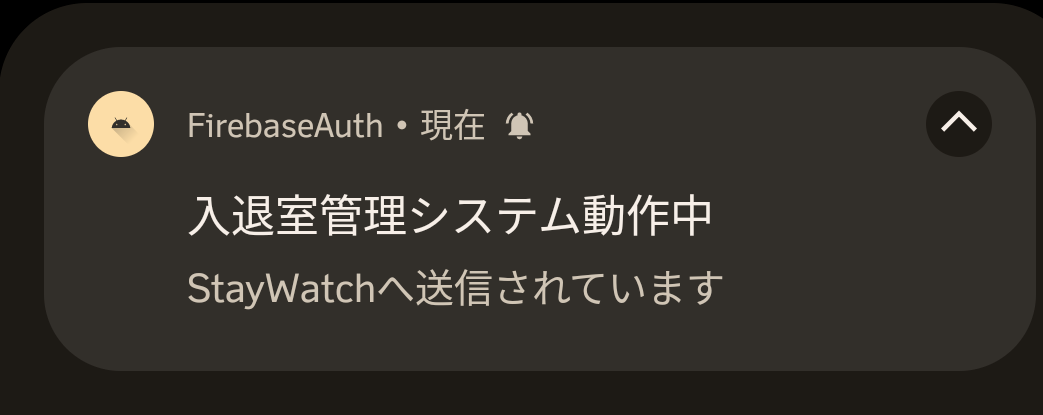
\includegraphics[width=14cm]{image/AppNofication.png}
  \caption{通知領域におけるビーコンの動作状況の表示}
  \label{fig:AppNofication}
\end{figure}


スマートフォンビーコンは基本的にバックグラウンドに常駐させる利用法を想定し実装した.
既存研究ではメンバに実デバイスによるビーコンを携帯させ,能動的な記録動作の必要がない.
スマートフォンのバックグラウンドに常駐させる方式は実デバイスによるビーコンと
同様に能動的な記録動作の必要がないため実デバイスによるビーコンと同等の利便性がある.
そのためバックグラウンドへの常駐がアプリケーション化の前提とした.
その点を踏まえて動作プラットフォームを選定した.
選定理由は技術調査をした際に,現状のiOSではフォアグラウンド動作はするもののバックグラウンド動作に制限がかかっており実デバイスによるビーコンと同等の利便性の担保が困難であると判明したため,対応プラットフォームをAndroidのみとした.

実装に伴い,アプリケーションのプログラムはKotlinを用い,Bluetooth関連の実装においてはAltBeaconというライブラリを利用した.
選定した理由としては,Android標準のライブラリについての情報が少なく,一部公式ドキュメントが削除されている中でAltBeaconに関する情報は多く提供されているからである.
ビーコン動作をする上で,Androidのプライバシ規則によって,バックグラウンド上でのユーザへの通知無しでの動作は禁止されている.
その点と,先述のスマートフォンが表示機能を持つ点を利用して 図\ref{fig:AppNofication}に示す通り通知領域上でビーコン動作中は常時表示する仕様とした.
この仕様によってAndroidのプライバシ規則を遵守している.
さらにユーザが入退室のたびにアプリの起動を行う必要がない実デバイスによるビーコンと同様の利便性を担保した.



ビーコンのアプリケーション化に伴い,管理者が実デバイスによるビーコンで行っていた登録作業をより簡略化した.
従来では管理者が新しいメンバが増えるたびにシステムにGoogleアカウント,名前,UUIDなどを登録し,割り当てられたUUIDを実デバイスによるビーコンに設定する作業を行っていた.
しかし先述のFirebaseによるログインを利用しメンバに紐づいているGoogleアカウントを用いて,スマートフォンビーコン上で利用するUUIDを自動で設定できるようにした.
図\ref{fig:AppSignIn}に示すサインインで管理者が登録したGoogleアカウントと一致する場合にログインを行う.その後APIからメンバの情報を受け取りUUIDをアプリ内部に設定する.
以降はログイン時に受け取ったUUIDを用いてビーコン動作を行う.
\begin{figure}[tbh]
  \centering
  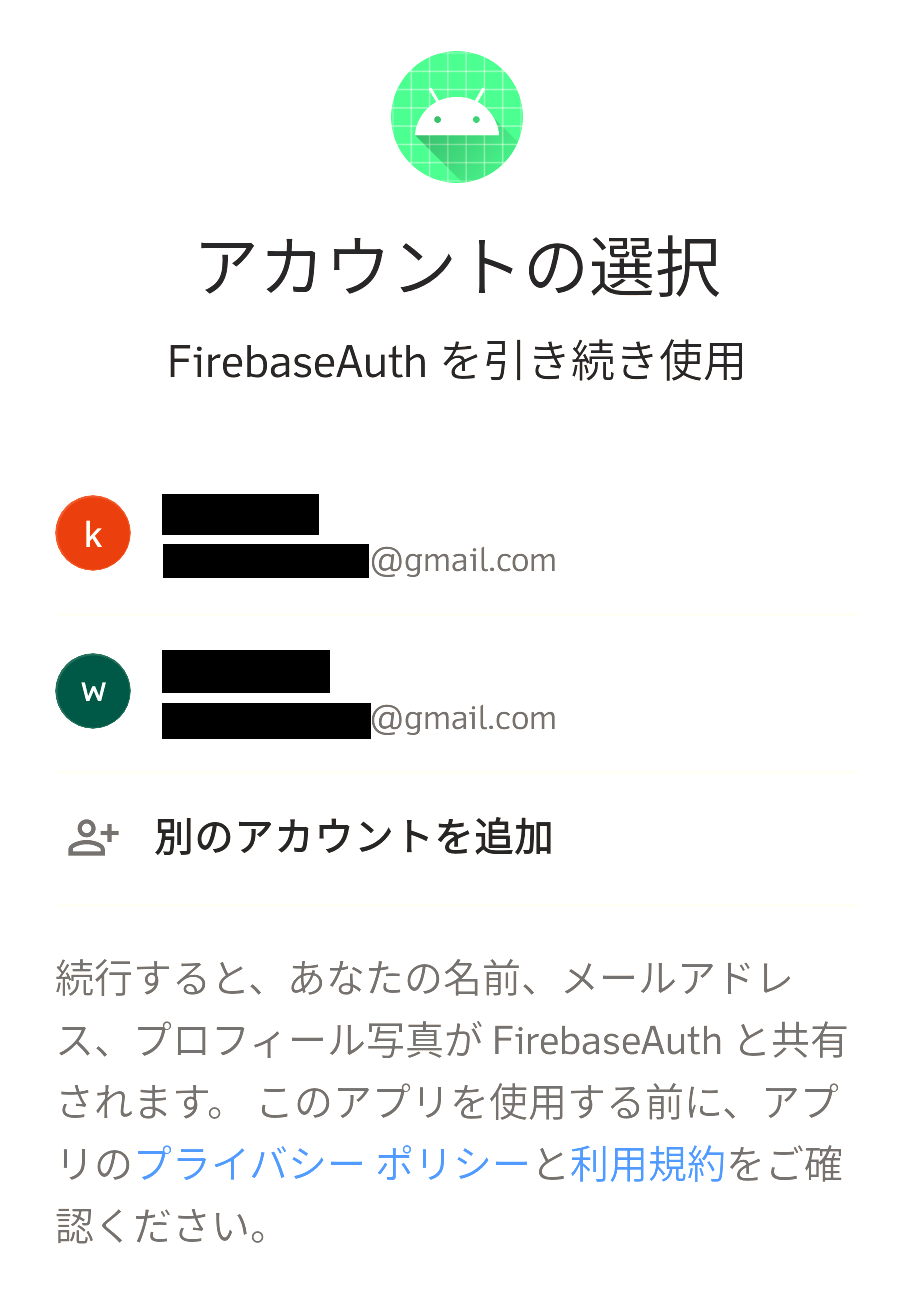
\includegraphics[width=6cm]{image/AppSignIn.png}
  \caption{アプリケーションのログイン画面}
  \label{fig:AppSignIn}
\end{figure}

% 画面の変更の写真を入れる
% \begin{figure}[tbh]
%   \centering
%   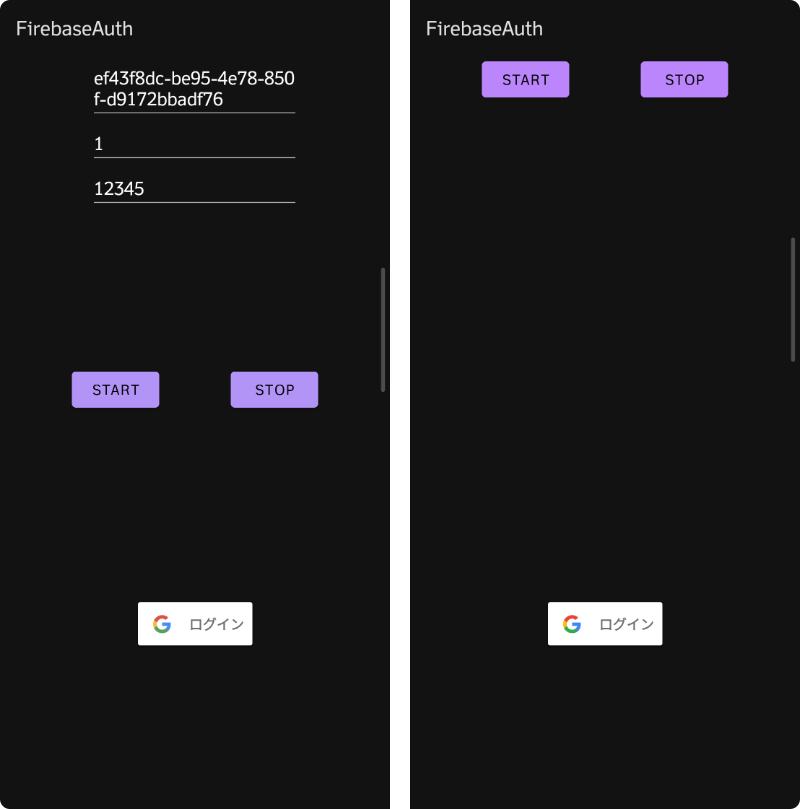
\includegraphics[width=9cm]{image/AppBeforeAfter.png}
%   \caption{メンバ向けアプリケーションにおける操作の簡略化}
%   \label{AppBeforeAfter}
% \end{figure}
% また図  X   研究初期はユーザから利用しているUUID,major,minorを編集できる仕様にしていたが,複雑な操作がユーザの利便性の向上につながらないと考え取り消した.
% あと,実デバイスによるビーコンでは管理者がユーザ登録を行ったあと紐づけたビーコンに一台ずつ対応したUUIDを割り当てていたが,スマートフォンビーコンならばウェブ上に登録されたユーザに紐づいたUUIDを持ってくる
% 4.2章が完成したときに整合性を取ろう!!!